\documentclass[tikz]{standalone}
    \usepackage{tikz}
    \usetikzlibrary{positioning, graphs}
    \usetikzlibrary{graphs.standard}
    \begin{document}
    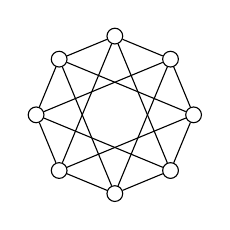
\begin{tikzpicture}
            [every node/.style={draw,circle,inner sep = 0mm, minimum size = 2mm}]
            \graph[clockwise, radius = 1cm, empty nodes]{subgraph C_n[n = 8, name = A]};
            
            \foreach \i [evaluate={\j=int(mod(\i+4,8)+1);}] in {1, 2, 3, 4, 5, 6, 7, 8}{
                \draw (A \i) -- (A \j);
            }
    \end{tikzpicture}
    \end{document}